\documentclass[conference]{IEEEtran}
\IEEEoverridecommandlockouts
% The preceding line is only needed to identify funding in the first footnote. If that is unneeded, please comment it out.
\usepackage{cite}
\usepackage{amsmath,amssymb,amsfonts}
\usepackage{algorithmic}
\usepackage{graphicx}
\usepackage{float}
\usepackage{textcomp}
\usepackage{xcolor}
\usepackage{url}
\usepackage{booktabs}
\def\BibTeX{{\rm B\kern-.05em{\sc i\kern-.025em b}\kern-.08em
    T\kern-.1667em\lower.7ex\hbox{E}\kern-.125emX}}
\begin{document}

\title{Efficiency Analysis of Image Compression Formats\\
\thanks{Eötvös Loránd University}
}

\author{\IEEEauthorblockN{1\textsuperscript{st} István Kiss}
\IEEEauthorblockA{\textit{Department of Programming Languages And Compilers} \\
\textit{Eötvös Loránd University}\\
Budapest, Hungary \\
ORCID: 0009-0002-9662-0134}
\and
\IEEEauthorblockN{2\textsuperscript{nd} Dr. Attila Kiss}
\IEEEauthorblockA{\textit{Department of Information Systems} \\
\textit{Eötvös Loránd University}\\
Budapest, Hungary \\
ORCID: 0000-0001-8174-6194}
}

\maketitle

\begin{abstract}
This paper investigates the efficiency of lossless photo compression algorithms, focusing on their potential benefits for data storage and image processing applications. Using the Kodak Image Suite, we evaluate multiple formats, including PNG, BMP, WEBP (lossless), and QOI (Quite OK Image format), by comparing their encoding and decoding speeds as well as compressed file sizes. Among these, QOI emerges as a standout, offering faster encoding times and smaller file sizes compared to more established formats like PNG, suggesting it could serve as a superior alternative. These improvements have significant implications for various applications: faster encoding could enhance photo capture rates on cameras and smartphones, while smaller file sizes could optimize storage on devices and cloud platforms, potentially saving costs and enabling more extensive datasets for AI training. The findings highlight the trade-offs between legacy and contemporary formats, emphasizing the practical advantages of adopting modern compression technologies in an increasingly data-driven landscape.
\end{abstract}
% HF 01 END



\begin{IEEEkeywords}
Image processing, Computer Graphics, Compression Algorithms
\end{IEEEkeywords}

\section{Introduction}
Image compression is a critical aspect of modern computing, playing a key role in data storage, transmission, and processing. With the increasing reliance on images in areas such as artificial intelligence, cloud storage, and personal devices, efficient compression methods are more important than ever. The ability to encode images quickly, decode them efficiently, and minimize storage requirements has the potential to improve system performance across a range of applications. For instance, faster encoding can enhance photo capture rates on devices like smartphones and cameras, while smaller file sizes can reduce storage costs and enable the handling of larger datasets in AI and machine learning workflows.

While lossy compression methods such as JPEG have long dominated the field for their ability to significantly reduce file sizes, lossless compression remains essential in scenarios where image quality must be preserved without compromise. Applications like medical imaging, archival storage, and professional photography often rely on lossless formats to maintain fidelity, ensuring that no data is lost during compression. This necessity underscores the continued relevance of evaluating and improving lossless compression techniques.

Historically, image compression formats have tended to evolve slowly, with many legacy formats being iteratively updated rather than replaced. Formats like PNG and BMP, for example, have remained widely used for decades, primarily due to their broad compatibility and ease of implementation. However, recent advancements in computational efficiency and algorithm design have enabled the development of newer formats that promise improved performance. One such example is the Quite OK Image (QOI) format, which aims to deliver faster encoding and decoding speeds while achieving competitive or better compression ratios compared to traditional lossless formats.

This study investigates the efficiency of several lossless image compression formats, including PNG, BMP, WEBP (lossless), and QOI, using the Kodak Image Suite as a benchmark dataset. The focus is on evaluating these formats in terms of encoding and decoding speeds as well as compressed file sizes. By comparing the performance of a newer format like QOI with established ones, this research seeks to determine whether adopting such a format could yield tangible benefits for modern applications.

One notable challenge in this exploration is the limited adoption of newer formats like QOI in mainstream software libraries. For example, while formats such as PNG and BMP are natively supported by Python's imageio library, testing QOI required the use of a specialized library. This lack of integration highlights the hurdles that newer formats face despite their technical advantages. Nonetheless, the trends toward smaller file sizes and greater efficiency make the exploration of such innovations increasingly relevant.

The findings of this paper aim to provide insights into whether transitioning to newer formats is worth the effort, particularly for applications where encoding speed, decoding efficiency, and file size optimization are paramount. By addressing these considerations, the study contributes to ongoing efforts to improve the performance of image compression systems in an increasingly data-driven world.

\section{Problem Statement}

With the rapid growth of digital media, efficient storage and transfer of images have become critical in various domains, from cloud storage and web applications to embedded systems and gaming. Traditional image compression formats like BMP and PNG offer established solutions but face limitations in balancing encoding/decoding speed and file size efficiency. Newer formats, such as WebP and QOI, claim to address these trade-offs by providing faster processing speeds or better compression ratios. However, their performance in practical scenarios remains underexplored, particularly in diverse application contexts.

This research aims to evaluate and compare these formats—BMP, PNG, WebP (lossless), and QOI—using key metrics: encoding time, decoding time, and file size. By identifying the strengths and weaknesses of each format, this study seeks to provide actionable insights into their suitability for different applications and to bridge the gap between theoretical claims and real-world performance.


\section{Dataset}
The dataset used for this study is the Kodak Image Suite\cite{dataset_kodak}, a collection of 24 high-resolution images widely utilized as a benchmark in image compression research. These images are well-suited for evaluating compression algorithms due to their variety in content, including diverse textures, colors, and levels of detail. This diversity ensures that the results obtained are not biased toward specific types of images and are representative of real-world scenarios.

\begin{figure}[htbp]
\centering
\includegraphics[width=\columnwidth]{MyPaper/figs/kodim23.png}
\caption{An example image from the dataset.}
\label{example_img_1}
\end{figure}

The Kodak Image Suite provides images in a lossless format, preserving their original quality. This characteristic is particularly important for this study, as it allows for a fair comparison of lossless compression methods. The images are typically 768 × 512 pixels in resolution, making them high enough in quality to stress test compression algorithms while remaining computationally manageable for experimentation.

The dataset was selected for its accessibility and widespread acceptance in the field. It provides a standardized basis for evaluating the performance of different compression formats, enabling comparisons that are consistent with prior research. Furthermore, the modest size of the dataset—24 images—makes it suitable for testing multiple algorithms without imposing excessive computational overhead.

For this study, the images were preprocessed by reading them into NumPy arrays to ensure compatibility with the libraries used for encoding and decoding operations. No further transformations were applied to the images to preserve their original characteristics and avoid introducing biases.

Overall, the Kodak Image Suite serves as a reliable and practical dataset for evaluating the efficiency of lossless image compression formats, providing a solid foundation for the analyses presented in this paper.


\section{Image Compression Formats}
This section explores the image compression formats evaluated in this study, detailing their history, compression techniques, applications, and current status. The formats are presented chronologically, beginning with the oldest.

\subsection{BMP (Bitmap Image File)}
The BMP format, also known as Bitmap Image File or Device Independent Bitmap (DIB), was introduced by Microsoft in 1986 as part of the Windows 2.0 operating system. It was designed to provide a simple, device-independent way to represent images on the screen. The format has remained largely unchanged since its inception, with its simplicity being its defining characteristic.

BMP primarily stores images as uncompressed pixel data, though some versions support Run-Length Encoding (RLE) compression. RLE reduces file size by encoding consecutive pixels of the same color as a single value and count. However, this approach is rarely used in practice due to its limited effectiveness. BMP files often lack advanced compression, making them much larger than other formats.

BMP files are primarily used in environments where compatibility and simplicity are paramount, such as in early graphical user interfaces, simple image editing, and hardware testing. However, due to their large file sizes, BMP has become less common in modern applications, largely replaced by more efficient formats.

BMP is no longer actively developed or maintained as a competitive format. Its last major update occurred with the release of Windows Bitmap specifications in the 1990s. It is still supported in many software libraries for backward compatibility.

\subsection{PNG (Portable Network Graphics)}
PNG was developed in 1995 by a working group led by Thomas Boutell as a response to licensing issues surrounding the GIF format, which required royalties for its patented Lempel-Ziv-Welch (LZW) compression. The first stable release, PNG 1.0, occurred in 1996, and the format became widely adopted as a free and open alternative.

PNG uses lossless data compression based on the Deflate algorithm, which combines LZ77 compression and Huffman coding. It also employs filtering techniques to preprocess image data, improving compression efficiency. This makes PNG ideal for storing images where quality preservation is critical.

PNG is widely used on the web for images requiring transparency, such as logos and icons, and for screenshots, where lossless quality is important. It has become the de facto format for lossless image storage in many applications.

PNG remains actively supported and is a standard in most software libraries and applications. The last stable specification was PNG 1.2, updated in 2004, though its usage has not declined.

\subsection{WEBP (Lossless)}
WEBP was introduced by Google in 2010 as a modern, open-source image format designed to reduce file size for faster web performance. Initially developed to support lossy compression, a lossless mode was added in 2012 to broaden its use cases.

WEBP lossless mode uses a combination of advanced techniques, including predictive coding and Huffman coding, to achieve high compression efficiency while preserving image quality. Its predictive algorithm encodes pixels based on the values of neighboring pixels, resulting in smaller file sizes than PNG in many cases.

WEBP is primarily used in web development, where smaller image sizes improve page loading times and reduce bandwidth usage. It is increasingly supported by major browsers and platforms, including Chrome, Firefox, and Edge.

WEBP is actively maintained by Google, with its last stable release, version 1.3.1, in June 2023. It continues to gain adoption in the web ecosystem due to its efficiency and versatility.

\subsection{QOI (Quite OK Image)}
QOI was introduced in 2021 by Dominic Szablewski as a lightweight, lossless image compression format. It was designed to be a simpler alternative to PNG, focusing on fast encoding and decoding speeds with reasonable compression efficiency.

QOI employs a run-length encoding (RLE)-like scheme combined with a custom hash-based lookup for pixel prediction. The format avoids complex preprocessing or entropy coding, trading some compression efficiency for significantly faster processing speeds.

QOI is particularly suited for scenarios where encoding and decoding speed is critical, such as in real-time applications, game development, and image processing pipelines. Despite its recent introduction, it has attracted interest due to its simplicity and performance advantages over legacy formats.

QOI is actively supported by its creator and the open-source community, with the latest stable release being version 1.0 in December 2021. However, it is not yet widely integrated into mainstream software libraries.

\section{Testing Framework}
The testing framework was implemented in Python, utilizing libraries such as imageio for handling .png, .bmp, and .webp (lossless) formats, and the qoi library for working with the .qoi format. To facilitate compatibility across these libraries, all images from the dataset were first read into NumPy arrays, as both imageio and qoi require this format for encoding and decoding operations.

To measure the performance of the compression formats, the time.time() method in Python was employed. For each image, the encoding process was timed by recording the start and end times surrounding the write operation to a file. The same approach was applied to the decoding process. This method yielded the encoding and decoding times in milliseconds. Additionally, the file size of the encoded image was recorded in bytes after each operation.


The metrics collected during the tests included:
\begin{itemize}
    \item Encoding Time: The time taken to compress an image into a specific format.
    \item Decoding Time: The time taken to decompress an image back into its original representation.
    \item File Size: The size of the compressed image in bytes.
\end{itemize}

Tests were conducted using Google Colab, configured to run exclusively on CPU to ensure consistent results. Although the tests were not repeated for multiple iterations, average results across all images in the dataset were calculated for each format, providing a representative performance summary.

All testing scripts and methods used in this framework have been made publicly available on GitHub\cite{github_repo} to promote reproducibility and transparency.

\section{Experimental Setup}
The experimental setup was designed to systematically evaluate the performance of the selected image compression formats using the Kodak Image Suite as the dataset.

Each image from the dataset was first converted into a NumPy array to ensure compatibility with the compression libraries. The same set of images was used for all formats to maintain consistency across tests.

For each format, the process began by encoding the image array into the respective compressed format, timing the operation to capture the encoding time. This was immediately followed by decoding the file back into a NumPy array, with the time for this operation also recorded. Finally, the size of the compressed file was measured in bytes.

The testing sequence was repeated for every image and compression format, resulting in a comprehensive set of performance data for encoding, decoding, and file size. All results were stored programmatically in arrays for further analysis and visualization.

The collected metrics were visualized using scatter plots and bar charts to identify trends and performance characteristics across the formats. These visualizations were generated within the same Python environment, ensuring seamless integration with the testing framework.

No additional baseline or validation checks were performed during testing, as the focus was solely on evaluating the relative performance of the formats under consistent conditions. Each test was conducted as a single iteration per image, aiming to provide an overview of average expected results for each format.

This straightforward experimental setup enabled efficient collection and comparison of performance metrics, laying the foundation for the analysis presented in subsequent sections of the paper.






\section{Results and Analysis}

In this section, we present the results of evaluating the four image compression formats --- PNG, BMP, WebP (lossless), and QOI (Quite OK Image format). The evaluation focused on three primary metrics: encoding time, decoding time, and encoded file size. To aid visualization and analysis, scatter plots and bar charts are included to illustrate the relationships and comparisons among these metrics. 

\subsection{Overview of Results}

Table \ref{tab:results} summarizes the average results for encoding time, decoding time, and encoded file size for each format. All time measurements are in milliseconds (ms), and file sizes are in kilobytes (KB).

\begin{table}[htbp]
    \centering
    \caption{Average Results for Each Compression Format}
    \label{tab:results}
    \begin{tabular}{|c|c|c|c|}
        \hline
        \textbf{Format} & \textbf{Enc. (ms)} & \textbf{Dec. (ms)} & \textbf{Size (KB)} \\
        \hline
        PNG & 222.4 & 28.4 & 664 \\
        \hline
        BMP & 4.4 & 4.6 & 1179.70 \\
        \hline
        WebP (Lossless) & 547.1 & 21.4 & 472.45 \\
        \hline
        QOI & 8.3 & 6.1 & 687.56 \\
        \hline
    \end{tabular}
\end{table}

\subsection{Encoding Performance}

Encoding performance reflects the time required to compress an image into the respective format. Among the tested formats:

\begin{figure}[H]
    \centering
    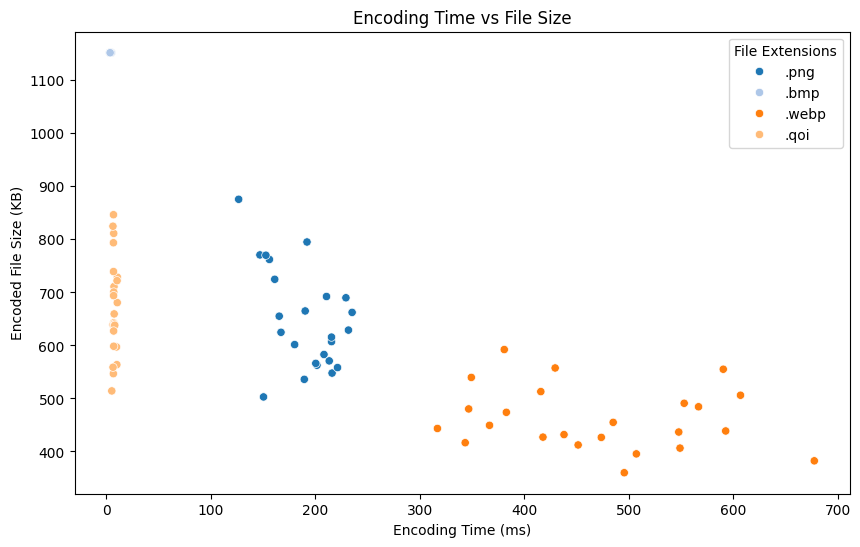
\includegraphics[width=\columnwidth]{MyPaper/figs/encoding_vs_file_size_scatter_plot.png}
    \caption{Scatter plot of encoding time vs file size for each image format.}
    \label{fig:encoding_scatter}
\end{figure}

\begin{itemize}
    \item \textbf{BMP}: BMP exhibited the fastest encoding time, with an average of 4.4 ms per image. Its simple raw data representation minimizes processing overhead, making it ideal for speed-critical tasks where file size is not a concern.
    \item \textbf{QOI}: QOI demonstrated excellent encoding performance at 8.3 ms on average. Its speed makes it suitable for applications such as real-time image processing and embedded systems.
    \item \textbf{PNG}: PNG encoding was relatively slow at 222.4 ms due to its complex lossless compression algorithm (DEFLATE). While effective for reducing file sizes, its slower performance limits use in time-sensitive applications.
    \item \textbf{WebP (Lossless)}: WebP recorded the slowest encoding time at 547.1 ms. Its advanced compression prioritizes storage efficiency but significantly increases computational requirements during encoding.
\end{itemize}

The relationship between encoding time and file size is illustrated in Figure \ref{fig:encoding_scatter}, while Figure \ref{fig:encoding_bar} provides a comparative view of average encoding times for each format.

\begin{figure}[htbp]
    \centering
    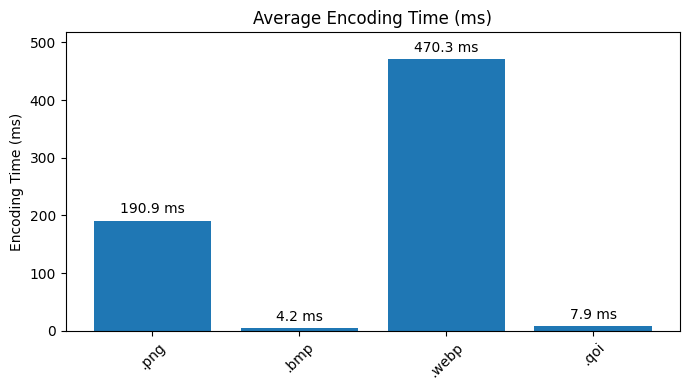
\includegraphics[width=\columnwidth]{MyPaper/figs/fig_average_encoding.png}
    \caption{Bar chart of average encoding time for each format.}
    \label{fig:encoding_bar}
\end{figure}

\subsection{Decoding Performance}

Decoding performance represents the time required to decompress an image back into a usable format. Key observations include:

\begin{figure}[H]
    \centering
    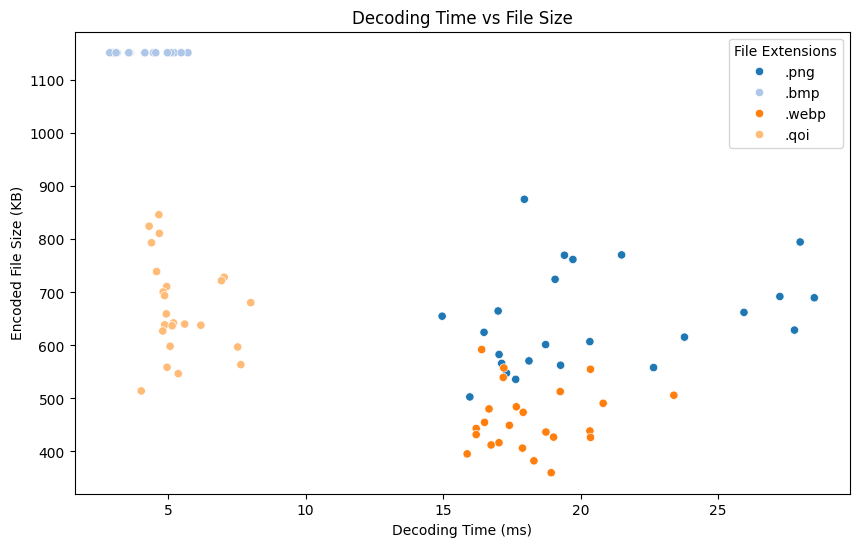
\includegraphics[width=\columnwidth]{MyPaper/figs/decoding_vs_file_size_scatter_plot.png}
    \caption{Scatter plot of decoding time vs file size for each image format.}
    \label{fig:decoding_scatter}
\end{figure}

\begin{itemize}
    \item \textbf{BMP}: BMP excelled in decoding speed, with an average of 4.6 ms. This, combined with its fast encoding, makes it a good choice for scenarios prioritizing speed over storage.
    \item \textbf{QOI}: QOI achieved efficient decoding at 6.1 ms, reinforcing its suitability for real-time applications.
    \item \textbf{WebP (Lossless)}: WebP showed competitive decoding performance at 21.4 ms, making it viable for read-heavy applications despite its slow encoding speed.
    \item \textbf{PNG}: PNG decoding was slower at 28.4 ms. This could pose limitations in applications where rapid image retrieval is essential.
\end{itemize}

Figure \ref{fig:decoding_scatter} presents a scatter plot of decoding time vs file size, and Figure \ref{fig:decoding_bar} provides a bar chart comparing average decoding times across formats.

\begin{figure}[htbp]
    \centering
    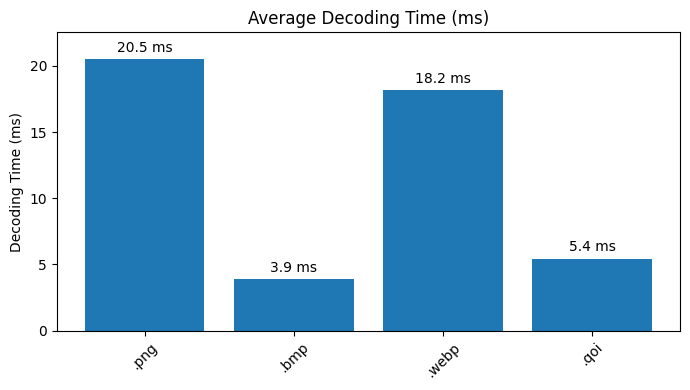
\includegraphics[width=\columnwidth]{MyPaper/figs/fig_average_decoding.png}
    \caption{Bar chart of average decoding time for each format.}
    \label{fig:decoding_bar}
\end{figure}

\subsection{File Size Efficiency}

File size efficiency is crucial for storage and data transfer. The results show:

\begin{itemize}
    \item \textbf{WebP (Lossless)}: WebP produced the smallest average file size at 472.45 KB, making it ideal for storage-constrained environments such as cloud services and mobile devices.
    \item \textbf{PNG}: PNG files averaged 664.23 KB, demonstrating strong compression capabilities for lossless formats. It remains suitable for applications prioritizing quality preservation.
    \item \textbf{QOI}: QOI files averaged 687.56 KB, balancing speed and compression. Its efficiency makes it a promising alternative to PNG in performance-critical scenarios.
    \item \textbf{BMP}: BMP files were the largest at 1179.70 KB, reflecting its uncompressed nature. BMP is recommended only for temporary storage where file size is not a concern.
\end{itemize}

Figure \ref{fig:file_size_bar} illustrates the average file sizes for each format.

\begin{figure}[htbp]
    \centering
    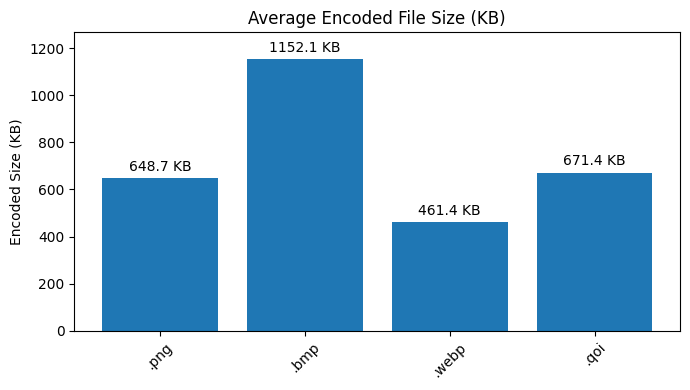
\includegraphics[width=\columnwidth]{MyPaper/figs/fig_average_file_size.png}
    \caption{Bar chart of average file size for each format.}
    \label{fig:file_size_bar}
\end{figure}

\subsection{Results Overview and Recommendations}

The results highlight significant trade-offs among the formats:

\begin{itemize}
    \item \textbf{BMP}: Best for speed-critical applications where storage constraints are not a priority.
    \item \textbf{PNG}: A versatile choice for lossless image storage with good compression and wide compatibility, though its slower performance limits its use in real-time scenarios.
    \item \textbf{WebP (Lossless)}: Optimal for applications requiring maximum file size reduction, such as cloud storage and bandwidth-sensitive environments. However, its slow encoding makes it less suitable for real-time encoding tasks.
    \item \textbf{QOI}: A modern, efficient alternative to PNG, offering competitive compression with superior encoding and decoding speeds. Ideal for embedded systems, games, and performance-critical workflows.
\end{itemize}

In conclusion, selecting the appropriate image format depends on the specific application requirements, balancing factors like speed, storage, and compatibility. These results provide valuable insights into making informed decisions for diverse use cases.






\section{Related Works}

\subsection{The JPEG still picture compression standard \cite{hf06001}}
The JPEG committee has established the first international standard for compressing continuous-tone still images, including both grayscale and color. It features two main methods: a DCT-based approach for lossy compression and a predictive method for lossless compression, with the widely used Baseline method as a key variant.

\subsection{The JPEG 2000 still image compression standard \cite{hf06002}} 
This article provides a detailed description of Part I of the JPEG 2000 standard, which is royalty-free to encourage broad adoption. The paper covers the standard's architecture, including tiling, multicomponent transformations, wavelet transforms, and entropy coding. It also discusses key features such as region-of-interest coding, scalability, and error resilience, and presents performance comparisons with existing standards.

\subsection{JPEG2000 Image Compression Fundamentals, Standards and Practice \cite{hf06003}}
The book provides a comprehensive reference on image compression, focusing on the JPEG2000 standard. It covers the fundamentals of image compression, a detailed description of the JPEG2000 standard, and practical guidelines for its implementation in both software and hardware, along with a discussion of other compression standards like JPEG and JPEG-LS.

\subsection{Overview of the High Efficiency Video Coding (HEVC) Standard \cite{hf06004}} 
High Efficiency Video Coding (HEVC) aims to deliver a significant compression improvement over existing video coding standards, targeting a 50\% reduction in bit-rate for the same perceptual video quality. This paper highlights the key technical features and innovations of the HEVC standard, which is being developed by the ITU-T Video Coding Experts Group and the ISO/IEC Moving Picture Experts Group.

\subsection{Overview of the H.264/AVC video coding standard \cite{hf06005}} 
H.264/AVC significantly improves rate-distortion efficiency and is designed for both conversational (e.g., video telephony) and non-conversational (e.g., streaming, broadcast) applications. This paper provides an overview of its technical features, profiles, and applications, as well as the history of the standardization process.

\subsection{Digital Image Compression Techniques \cite{hf06006}} 
This tutorial text introduces essential techniques for reducing the bit-rate of digital images, covering both lossless and lossy compression methods. It provides detailed descriptions of various algorithms, including the JPEG baseline algorithm, and compares their performance with reconstructed images, addressing quality, bit-rate, complexity, and error susceptibility.

\subsection{iWave: CNN-Based Wavelet-Like Transform for Image Compression \cite{hf06007}} 
The iWave framework uses a convolutional neural network (CNN) to design wavelet-like transforms for natural image compression, overcoming the limitations of traditional wavelets. By adopting a lifting scheme with a CNN prediction filter, iWave achieves better compression performance compared to JPEG-2000, reducing BD-rates by up to 27% when optimized for specific textures.

\subsection{End-to-end optimized image compression \cite{hf06008}} 
This method introduces an image compression approach that combines a nonlinear analysis transformation, uniform quantization, and a nonlinear synthesis transformation, optimized using stochastic gradient descent. The technique outperforms standard compression methods like JPEG and JPEG-2000 in rate-distortion performance, while offering superior visual quality at all bit rates, as validated by objective MS-SSIM metrics.

\subsection{Conditional probability models for deep image compression \cite{hf06009}} 
This paper introduces a method to navigate the rate-distortion trade-off in image compression auto-encoders by using a context model, a 3D-CNN that learns a conditional probability model of the latent representation. The approach results in a state-of-the-art image compression system, as demonstrated by experiments using MS-SSIM, outperforming previous methods based on convolutional auto-encoders.

\subsection{Lossy image compression with compressive autoencoders \cite{hf06010}} 
This paper introduces a method to optimize autoencoders for lossy image compression, addressing challenges in flexibility and efficiency. The approach shows that minimal adjustments to the loss function can enable deep autoencoders to compete with JPEG 2000 and outperform recent RNN-based methods, while maintaining computational efficiency through a sub-pixel architecture suitable for high-resolution images.

\subsection{Real-time adaptive image compression \cite{hf06011}} 
This paper presents a real-time image compression algorithm that outperforms existing codecs like JPEG, JPEG 2000, WebP, and BPG, achieving significantly smaller file sizes while maintaining high-quality reconstructions. The method uses an autoencoder architecture with pyramidal analysis, adaptive coding, and adversarial training, and is optimized for fast encoding and decoding, with GPU processing times around 10ms per image.

\subsection{Variable rate image compression with recurrent neural networks \cite{hf06012}} 
This paper proposes a novel framework for variable-rate image compression using convolutional and deconvolutional LSTM recurrent networks, aimed at improving thumbnail compression for mobile devices. The method allows for progressive image reconstruction with better visual quality and smaller file sizes than standard compression algorithms like JPEG, JPEG2000, and WebP, achieving reductions in storage size by 10% or more on a benchmark of 32×32 thumbnails.

\subsection{Improved lossy image compression with priming and spatially adaptive bit rates for recurrent networks \cite{hf06013}} 
This paper presents a method for lossy image compression using recurrent, convolutional neural networks that outperforms traditional codecs like BPG, WebP, JPEG2000, and JPEG in terms of MS-SSIM. Key improvements include training with a pixel-wise SSIM-weighted loss, modifying the recurrent architecture for better spatial diffusion, and incorporating a spatially adaptive bit allocation algorithm to efficiently encode complex image regions, achieving state-of-the-art results on Kodak and Tecnick image sets.

\subsection{Generating high fidelity images with subscale pixel networks and multidimensional upscaling \cite{hf06014}} 
The paper introduces the Subscale Pixel Network (SPN), a conditional decoder architecture for generating high-fidelity images. SPN tackles the challenges of encoding large image contexts and preserving both global coherence and fine details. The authors use Multidimensional Upscaling to generate large images and achieve state-of-the-art performance in unconditional image generation on datasets like CelebA-HQ and ImageNet, setting new benchmarks for high-quality, large-scale image generation.

\subsection{Variable rate deep image compression with a conditional autoencoder \cite{hf06015}} 
This paper introduces a variable-rate image compression framework using a conditional autoencoder. Unlike traditional methods that require separate networks for different compression rates, the proposed model uses two rate control parameters—the Lagrange multiplier and quantization bin size—to adjust the compression rate. Experimental results show that this approach achieves a better rate-distortion trade-off than traditional codecs like JPEG2000 and BPG, and competes favorably with state-of-the-art learned models.

\subsection{Rethinking Lossy Compression: The Rate-Distortion-Perception Tradeoff \cite{hf06016}} 
This paper extends the classical rate-distortion theory to incorporate perceptual quality by introducing a three-way tradeoff between rate, distortion, and perceptual quality. The study shows that prioritizing perceptual quality typically raises the rate-distortion curve, necessitating a tradeoff between rate or distortion. The authors provide closed-form calculations for a Bernoulli source and demonstrate the tradeoff visually using a toy MNIST example.

\subsection{Overview of the Versatile Video Coding (VVC) Standard and its Applications \cite{hf06017}} 
The VVC standard, finalized in 2020, delivers significant bit rate reductions of up to 50\% compared to HEVC and 75\% compared to AVC, while supporting a broad range of applications, including high-resolution video, high dynamic range, and immersive 360° video. The paper highlights the versatility of VVC for emerging media formats and applications such as adaptive streaming, ultralow-delay streaming, and multilayer coding. Early implementations demonstrate that VVC is ready for real-world deployment.

\subsection{End-to-End Learnt Image Compression via Non-Local Attention Optimization and Improved Context Modeling \cite{hf06018}} 
This paper presents an advanced learned image compression method using a deep neural network-based variational auto-encoder (VAE) with Non-Local Attention and Improved Context modeling (NLAIC). The approach integrates non-local operations and attention mechanisms for adaptive bit allocation, enhances entropy modeling with 3D CNN-based autoregressive contexts, and offers computational and memory optimizations for practical deployment. The proposed model outperforms existing compression methods such as BPG, JPEG2000, and JPEG on the Kodak and Tecnick datasets with superior compression efficiency, as measured by both PSNR and MS-SSIM.

\subsection{Video Compression - From Concepts to the H.264/AVC Standard \cite{hf06019}} 
This paper reviews the evolution of digital video compression techniques, focusing on the key elements contributing to modern video codecs' rate-distortion performance. The authors explain the integration of motion representation, intra-picture prediction, and waveform coding in the design of video compression standards, culminating in the H.264/AVC standard. The paper provides a comprehensive understanding of the development and application of these technologies in the field of video compression.

\subsection{Full Resolution Image Compression with Recurrent Neural Networks \cite{hf06020}} 
This paper presents a set of full-resolution lossy image compression methods based on recurrent neural networks (RNNs), achieving variable compression rates without requiring retraining. The architectures consist of an RNN-based encoder-decoder, binarizer, and entropy coding network, with improvements of 4.3\%-8.8\% in AUC over previous methods. The proposed approach outperforms JPEG in most bitrates on the Kodak dataset, with and without entropy coding.


\section{Conclusions}

This paper evaluated four lossless image compression formats—BMP, PNG, WebP (lossless), and QOI—by measuring their encoding and decoding times, as well as file size efficiency. Through extensive testing and analysis, we highlighted the trade-offs between these formats, emphasizing their strengths and limitations in terms of performance and storage.

The results demonstrated that BMP, while excelling in speed due to its lack of compression, produces significantly larger file sizes, limiting its practical use in modern storage-constrained environments. PNG, a widely adopted lossless format, provides a good balance between file size efficiency and performance but falls short in encoding and decoding speed compared to newer alternatives. WebP (lossless) exhibited the smallest file sizes, making it ideal for bandwidth-sensitive applications, though its slow encoding performance may restrict its use in time-critical tasks. Finally, QOI emerged as a promising alternative, delivering competitive file sizes with significantly faster encoding and decoding speeds, highlighting its potential for real-time and resource-limited applications.

The addition of visualizations, including scatter plots and bar charts, offered a clearer understanding of how these formats compare across key metrics. The analysis underscored the importance of selecting an image compression format based on specific use-case requirements, whether the priority is speed, storage efficiency, or a balance of both.

This research also identified areas for further exploration. Testing lossy compression formats alongside their lossless counterparts and revisiting emerging algorithms like JPEG XL could provide a more comprehensive understanding of image compression technologies. Additionally, conducting real-world application tests would offer deeper insights into their practical performance under diverse operational constraints.

In conclusion, while no single format excels in all aspects, the findings of this study provide valuable guidance for selecting the most suitable image compression format for various scenarios. By continuing to explore and refine these technologies, researchers and practitioners can better address the evolving needs of image storage and transmission in a data-driven world.

\section{Future Works}

This study has provided a comprehensive evaluation of four prominent image compression formats in their lossless configurations, focusing on encoding and decoding performance, as well as file size efficiency. However, several avenues for further research remain unexplored and could significantly enhance the understanding and applicability of image compression technologies.

Firstly, the inclusion of lossy formats in future studies could provide a more holistic view of image compression. Lossy formats such as JPEG and lossy WebP are widely used in scenarios where file size reduction is paramount, and a small loss in quality is acceptable. Comparing these formats with lossless ones under similar testing frameworks could yield valuable insights into their trade-offs and best-use cases.

Another promising area is the exploration of emerging image compression algorithms, such as JPEG XL. This algorithm, which supports both lossy and lossless compression, shows potential as a next-generation image format. However, due to its developmental status and limited library support, this study was unable to include JPEG XL in the evaluation. Future work could revisit JPEG XL as it matures, leveraging improved tools and libraries to conduct robust performance evaluations.

Additionally, while this study relied on controlled tests to measure encoding/decoding times and file sizes, future research could focus on more application-specific scenarios. For instance, real-life applications such as image storage for web platforms, cloud environments, or embedded systems could provide deeper insights into how these formats perform under practical constraints, including bandwidth limitations and system resource availability.

By addressing these gaps, future studies could further refine the understanding of image compression technologies and provide actionable recommendations for diverse real-world applications.


\bibliographystyle{ieeetr}
\bibliography{mypaper_references}

\vspace{12pt}

\end{document}
